% !TeX root = ../thesis.tex

\chapter{Methodology}
\label{sec:concepts}
\section{Datasets}
\subsection{KITTI Dataset}
In this paper, proposed attacks are conducted on the KITTI object detection dataset\cite{geiger_vision_2013}, which is a widely used benchmark dataset for adversarial attack research. In the KITTI 3D object detection benchmark, point clouds dataset is composed of a trainval set with 7481 training samples and a test set containing 7518 samples, involving 80256 labeled objects in total. Object class is provided in the dataset, where 'car', 'pedestrian' and 'cyclist' are the main concerned classes in the object detection studies. In addition, a leaderboard of detection method is published and continually updated on the KITTI website\cite{KITTI}, in which average precision is the main indicator to evaluate detection performance on the three main categories. Three difficulty levels "Easy, moderate, hard" are used to evaluate the detector, depending on the occlusion and truncation. More explanation of evaluation metrics will be provided in section \(\ref{evaluation Metrics}\).

\subsection{DENSE Dataset}
\textit{Autolabeling} 

Piewak et al.\cite{piewak_boosting_2018} proposed autolabeling method for labeling point clouds with classes. It uses camera and LiDAR installed with minimum instance to record the scenes simultaneously. Then uses the semantic segmentation network\cite{cordts_understanding_nodate}, which performs good at that time, trained on Cityscapes\cite{cordts_cityscapes_2016} for image segmentation. For point projection right to the reference camera plane, they proposed ego-motion correction. The general process is shown in Figure \(\ref{fig:Autolabeling}\).
\begin{figure}[!htbp]
\centering
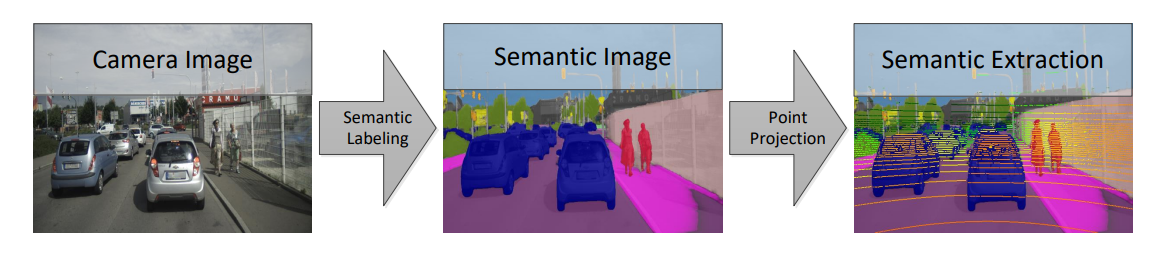
\includegraphics[scale=0.5]{Graphics/Autolabeling.png}
\caption{Autolabeling process. Segmentation network to do semantic segmentation in images and point projection to align pixels and point clouds and finish the labeling.\cite{piewak_boosting_2018}}
\label{fig:Autolabeling}
\end{figure}
\textit{DENSE\cite{DENSE}}

DENSE is a dataset in Ulm University, which seek to focus on how adverse weather influence the autonomous driving perception system. It creates the datasets under several adverse weather like fog,snow and rain. Heizler et al.\cite{heinzler_cnn-based_2020} followed the autolabeling process to gives the each point cloud a weather class. In In Figure \(\ref{fig:DENSE Dataset}\), the result of autolabeling is shown in right graph. Fog, rain and clean class have shown in different colors. Cause DENSE dataset includes many subsets. We only used the subset from Heizler's work. The subset uses 4 chamber to record point clouds of car, pedestrian and etc. under man-made weather for training and testing. They also have a on road dataset for further testing. This subset is good to observe the specialty of point clouds under different weather and simulate point clouds under adverse weather with point clouds under clean weather.

\begin{figure}[!htbp]
\centering
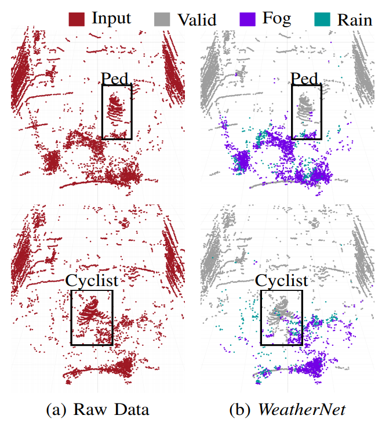
\includegraphics[scale=0.5]{Graphics/DENSE.png}
\caption{DENSE Dataset}
\label{fig:DENSE Dataset}
\end{figure}
\section{Evaluation Metrics}
\label{evaluation Metrics}
\subsection{KITTI}
\subsubsection{3D Bounding Box}
In object detection task, bounding box is an imaginary rectangle to mark the spatial location of the objects of interest. In 2D image detection, a bounding box can be determined by two methods, one is two-corner representation, rendered by the coordinates \(xy\) of the upper-left corner \((x_{min},y_{max})\) and the lower-right corner \((x_{max},y_{min})\), and another commonly used method is center-width-height representation, described by the bounding center center coordinates \((x,y)\) and the box width and height. 

3D bounding box annotations, including 3D size described in length, width and height and object’s rotation and translation, are provided for each object in the KITTI dataset\cite{geiger_vision_2013}. An illustration of 3D bounding box coordinates is in Figure \(\ref{fig:3D bounding box coordinate system}\). Specifically, under the assumption that the observed objects are pinned to the ground, only yaw angle is considered in rotation, and roll and pitch angles are assumed to be zero relative to the ground plane. The coordinates of 8 vertices of the 3D bounding box can be calculated by seven parameters, namely length, width, height, object center coordinates (x,y,z) and rotation angle, realizing the parameterization of 3D bounding box. 

\begin{figure}[!htbp]
\centering
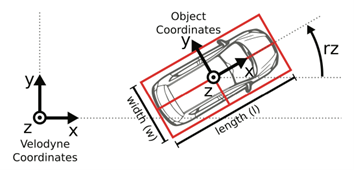
\includegraphics[scale=1]{Graphics/3D bounding box coordinate system.png}
\caption{3D bounding box coordinate system}
\floatfoot{This figure illustrates some parameters of 3D bounding box from the top view. Object coordinates are defined by the center point at the bottom of 3D bounding box, of which the coordinate system is constructed with respect to the LiDAR coordinate system. \(R_{z}\) is yaw angle representing the rotation. 3D size is determined by width(\(w\)), length(\(l\)) and height(\(h)\), which is not shown in the top view.\cite{geiger_vision_2013} }
\label{fig:3D bounding box coordinate system}
\end{figure}

\subsubsection{\acrshort{iou}}
Intersection over union(\acrshort{iou}) is an indicator showing the similarity of the ground truth bounding box and the detected bounding box, which is equal to the proportion of bounding box intersection to the union. It can be formulated as following:

\begin{equation}
          IoU_{b_{1},b_{2}} = \frac{A(b_{1}\cap b_{2})}{A(b_{1}\cup b_{2})} 
\end{equation}
Where \(A(\cdot)\) denotes the area and b means the bounding box. When \acrshort{iou} is larger than the threshold, it can be counted as positive. In the KITTI, \acrshort{iou} \(\geq\) 0.7 is required in the detection of cars, while \acrshort{iou} \(\geq\) 0.5 is accepted when recognizing pedestrians and cyclists.

\subsubsection{Average Precision}
Average precision (\acrshort{ap}) is a well-established indicator and is used to evaluate the detection performance in the KITTI. Following the PASCAL \acrshort{voc} criteria \cite{everingham_pascal_2010}, \acrshort{ap} is determined by the precision-recall curve. Precision describes how accurate the prediction is and recall measures how good you can find the positive. Specifically, precision is equal to the proportion of correct detections in all detections produced by the detector, and recall means the ratio of successful detections to all ground truth objects. The mathematical definitions are as following:
\begin{equation}
\label{precision}
          Precision = \frac{TP}{TP+FP}
\end{equation}
\begin{equation}
\label{recall}
          Recall = \frac{TP}{TP+FN} 
\end{equation}
Where \(TP\) represents true positive, implying the ground truth is present and model successfully detect the object. \(FP\) is false positive, indicating a detection when the ground truth is not present. \(FN\) means false negative, signifying the ground truth is present but not being detected by the detector.

From function \((\ref{precision})\) and \((\ref{recall})\), precision and recall are both between 0 and 1. Discretizing recall value uniformly into 11 equal-spaced points, 0,0.1,0.2,...,1. a fixed recall value set is defined. For any recall \(r^{'}\geq r\), we replace the precision value for r with maximum precision. Average precision is computed as the average of maximum precision value of the 11 recall values\cite{everingham_pascal_2010}, as function (\(\ref{AP}\)) and average precision always falls within 0 and 1.
\begin{equation}
\label{AP}
\begin{split}
    AP &= \frac{1}{11} \sum\limits_{r\in\{{0,0.1,...,1}\}} AP_{r} \\
    &=\frac{1}{11} \sum\limits_{r\in\{{0,0.1,...,1}\}} p_{interp}(r)\\
    where  \\
    &p_{interp}(r) = \max\limits_{r^{'}\geq r}p(r^{'})
\end{split}
\end{equation}
 
To promote fair comparison of the results, KITTI changed the AP definition using 40 recall positions to replace the 11 recall positions from Oct.2019\cite{KITTI,simonelli_disentangling_2019}. 
\subsubsection{Average Orientation Similarity}
\acrshort{aos}(Average Orientation Similarity) is the key 3D metric used in the KITTI dataset to evaluate the performance of detecting objects and assessing 3D orientation jointly\cite{geiger_are_2012}. Similar to the structure of \acrshort{ap}, \acrshort{aos} is the mean value of maximum normalized cosine similarity of 11 recall values\footnote{40 recall positions instead of 11 recall positions are used to calculate \acrshort{aos} after Oct.2019} and is defined as following:
\begin{equation}
    AOS = \frac{1}{11} \sum\limits_{r\in\{{0,0.1,...,1}\}}  \max\limits_{r^{'}\geq r}s(r^{'})
\end{equation}
Where \(s(\cdot)\) of a specific recall represents the orientation similarity, which is a normalized variant of the cosine similarity and is defined as:
\begin{equation}
    s(r) = \frac{1}{\abs{ D(r)}} \sum\limits_{i\in D(r)}  \frac{1+cos\Delta_{\theta}^{(i)}}{2} \delta_{i}
\end{equation}
Where \(D(r)\) is a set containing all object detections at a specific recall rate, delta describes the angle difference between estimated orientation and the ground truth orientation of the detection i. \(\delta_{i}\) is a parameter to penalize multiple detections to a single object and is determined by the overlapping of the bounding box. \(\delta_{i}\) is assigned to 1 when the detection i can be allocated to a ground truth bounding box(\acrshort{iou}\(\geq\)0.5), otherwise \(\delta_{i}\) is equal to 0.




\textit{Metric for adversarial attacks on LiDAR-based object detector}
As the simple evaluation metric in attacks\cite{xie_adversarial_2017,liu_adversarial_2019,li_robust_2019,zhang_towards_2019,wei_transferable_2019} under image object network, drop of AP of detection model could be used as the metric for effort of adversarial attacks. So we also pick the drop of AP score as our metric for evaluate the adversarial attack under LiDAR-based object detector.
\subsection{DENSE}
\section{Target LiDAR Detector Models}
\subsection{SECOND}
Sparsely Embedded Convolutional Detection (\acrshort{second}) is proposed by Yan et al. for LiDAR-based detection\cite{yan_second_2018}. \acrshort{second} detector is composed of three main components: a voxel feature extractor, a sparse convolutional layer and an \acrshort{rpn}(region proposal network). The first step is to convert raw point clouds into voxel features and coordinates, then a voxel feature extractor including two voxel feature encoding layers and a fully connected network is utilized to transfer input features into C-dimensional output features, where C is the number of output channels. Afterwards, sparse convolutional layer is used to learn z-axis information and transfer the sparse 3D information into a 2D \acrshort{bev} image. In the final phase, an \acrshort{rpn} incorporated three stage convolutions is used to predict the class, regression offsets and direction. 
\begin{figure}[!htbp]
\centering
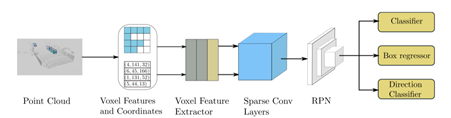
\includegraphics[scale=1]{Graphics/SECOND.png}
\caption{\acrshort{second} detector structure}
\floatfoot{This flowchart represents the structure of \acrshort{second} detector. The input of the detector is a raw point cloud. Voxel features and coordinates converted from the raw point clouds are firstly processed by the feature extractor. Later, a sparse \acrshort{cnn} is applied to reshape 3D data into image-like 2D information and \acrshort{rpn} is used to generate prediction lastly.}
\label{fig:SECOND}
\end{figure}
\subsection{PointPillar}
PointPillars is a novel encoder introduced by Lang et al.\cite{lang_pointpillars_2019}, which can utilize only 2D convolutional layers to achieve end-to-end learning. The procedure of PointPillars is illustrated in Figure \(\ref{fig:PointPillars}\). Pillar Feature Net, Backbone and Detection Head are the three main components in PointPillars. At the beginning, LiDAR point clouds are converted to the stacked pillars tensor, and then a simplified version of PointNet\cite{qi_pointnet_2017} is created to learn features from the stacked pillars, the encoded features are scattered back to produce a 2D pseudo image to be used in the backbone, all these works are conducted in the pillar feature net. The backbone contains a 2D CNN to process features into high spatial resolution and produce a final output which is a concatenation of all features. The detection head is a single shot detector to detect and regress the 3D bounding box.
\begin{figure}[!htbp]
\centering
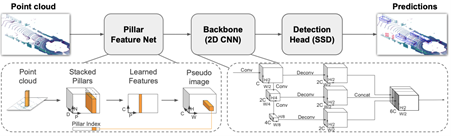
\includegraphics[scale=1]{Graphics/PointPillars.png}
\caption{PointPillars Network}
\floatfoot{This figure demonstrate the structure of PointPillars network. Raw point clouds are converted into a sparse pseudo image in the pillar feature net. Then the pseudo image is processed by the backbone, which is a 2D convolutional network, into a high level representation. At last the detection head is used to perform 3D detection.}
\label{fig:PointPillars}
\end{figure}
\subsection{PointRCNN}
PointRCNN is a two-stage 3D object detection approach proposed by Shi et al.\cite{shi_pointrcnn_2019}. Stage 1 is a novel strategy to generate 3D proposals in a bottom-up manner directly from point cloud, by learning point-wise features to segment the whole scene point clouds into foreground and background points. Compared with other existing methods, this proposal generation method constrains the search space and enhances the efficiency. Subsequently, a region of interest pooling operation is conducted to learn more semantic features and local spatial information of those proposals. Then the pooled points of each proposal are transformed into canonical coordinates and combined with the pooled features along with the segmentation mask to be fed into the network for further refinement, including 3D bounding box locations and foreground object confidence.
\begin{figure}[!htbp]
\centering
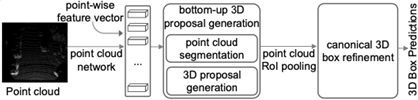
\includegraphics[scale=1]{Graphics/PointRCNN.png}
\caption{PointRCNN Architecture}
\floatfoot{This graph shows the structure of PointRCNN. A point cloud network is used to learn point-wise features and produce a feature vector. Then a bottom-up scheme is used to generate 3D bounding box proposals from the segmented foreground points. After performing an \acrshort{roi} pooling, the pooled points and corresponding features of each proposal are transformed into canonical coordinate for further refinement.}
\label{fig:PointRCNN}
\end{figure}
\subsection{Part-\(A^{2}\)}
Shi et al. extend their preliminary work PointRCNN to a novel network Part-\(A_{2}\)\cite{shi_points_2020}. 
Part-\(A_{2}\) comprises two stages: part-aware stage and part-aggregation stage. The task of part-aware stage is to predict intra-object part locations and learn point-wise features, and part-aggregation stage mainly contributes to part information aggregation and box refinement. An overview of the Part-A2 framework is displayed in Figure \(\ref{fig:PartA2}\). To be specific, 3D Point clouds are fed into the encoder-decoder network and transformed into feature maps. Considering different scenarios, two strategies are used to generate proposals, where anchor-based strategy can achieve high recall rates at the expenses of computation and memory cost while anchor-free strategy is more memory efficient. By fully utilizing part supervision from the ground-truth box, intra-object part location information are predicted and high-quality proposals are generated in the part-aware stage. Subsequently, via \acrshort{roi}-aware point cloud pooling module, intra-object part locations within the same proposal are grouped. With the aggregated spatial information, convolutional network is utilized to rescore the box proposals and refine the box locations. 

\begin{figure}[!htbp]
\centering
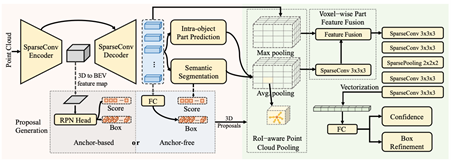
\includegraphics[scale=0.8]{Graphics/Part-A2.png}
\caption{Framework of Part-\(A_{2}\)}
\floatfoot{The left orange part illustrates the work in part-aware stage. Point clouds data are fed in to the network, which learns the point-wise features for semantic segmentation and estimation of the intra-object part locations. Two strategies anchor-free and anchor-based are used to generate 3D proposals. The right green part shows how part-aggregation stage operates. An \acrshort{roi}-aware pooling is performed to aggregating information within 3D proposals, Sparse \acrshort{cnn}s and sparse pooling are applied in the part-aggregation stage to produce accurate confidence prediction and box refinement.}
\label{fig:PartA2}
\end{figure}
\subsection{PointVoxel-RCNN}
A new contribution from Shi et al is PointVoxel-RCNN(PV-RCNN), which is an deeply intergrated network of both voxel-based and PointNet-based network\cite{shi_pv-rcnn_2021}. Two transformation steps are proposed: voxel to keypoint encoding step and keypoint to grid \acrshort{roi} feature capture step. More specific procedures are shown in Figure 8. After going through voxelization, processed point clouds are fed into 3D sparse convolutional network to learn multi-scale voxel-wise information and 3D proposals are generated using RPN. In addition, a set of keypoints are selected from the raw point clouds by \acrshort{fps} (furthest point sampling) method. A novel voxel set abstraction module is introduced to intergrate the voxel-wise features learned at convolution neural layers into selected keypoints. After the keypoint weighting module, keypoint features combined with 3D box proposals(\acrshort{roi}) are combined in the \acrshort{roi}-grid pooling module to capture proposal-specific features. Using the \acrshort{roi} feature of each proposal, a refine network is performed in order to generate box refinement and confidence prediction.
\section{Attack and Defense Methods}
\subsection{\acrshort{fgsm} and FGSM Variants}
\subsubsection{\acrshort{fgsm}}
Fast gradient sign method (\acrshort{fgsm}) is proposed by Goodfellow et al, which is a one-step attack algorithm founded on the idea to maximize loss function subject to an upper bound of the perturbation.( Explaining and harnessing adversarial examples ). Panda example is a well-known classical adversarial attack with FGSM approach, which is shown in Figure \(\ref{fig:FGSM}\).  Formally, FGSM can create an attack as following:
\begin{equation}
          x^{'} = x + \epsilon \cdot sign(\nabla_{x}J(\theta,x,y)) 
\end{equation}
Where x is the benign data point, \(x^{'}\) is the perturbed data point, \(\theta\) are parameters of the model, y represent ground truth labels, \(J(\theta,x,y)\) is loss function, \(\nabla_{x}J(\theta,x,y)\) denotes the gradient of loss function taken with respect to the input data x, and the gradients can be efficiently computed by backpropagation. The sign of the gradient is the perturbation direction. \(\epsilon\) represents the magnitude of the perturbation.
\begin{figure}[!htbp]
\centering
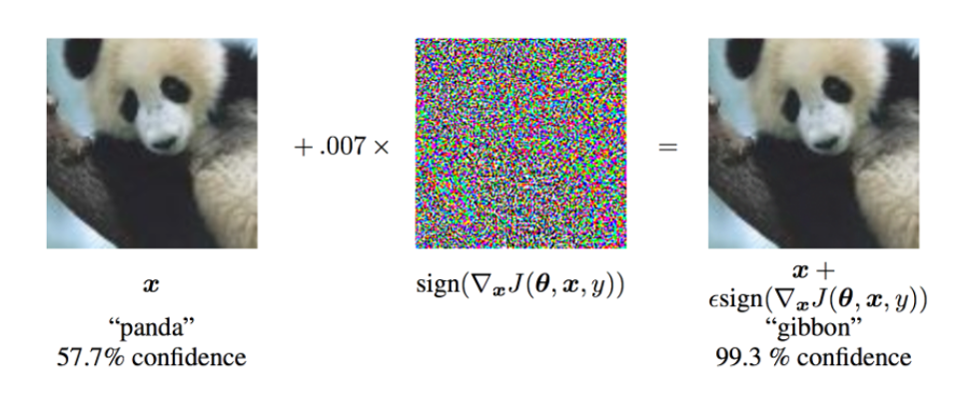
\includegraphics[scale=0.5]{FGSM.png}
\caption{An adversarial attack by FGSM}
\floatfoot{The adversarial sample is crafted by applying FGSM to GoogLeNet\cite{szegedy_going_2015}. By adding imperceptible perturbation, where the \(\epsilon\) is 0.007, the classifier incorrectly recognizes the panda as a gibbon with high confidence.\cite{goodfellow_explaining_2015}}
\label{fig:FGSM}
\end{figure}

\subsubsection{FGSM Variants}
\paragraph{Iterative FGSM (IFGSM) and \acrshort{pgd}} 
One drawback of FGSM is that the perturbed data points might be unbounded, which is physically prohibited in image classification problems. To solve this issue,  Kurakin et al.\cite{kurakin_adversarial_2017} introduce an improved version by iteratively apply \acrshort{fgsm} multiple times(T) with a step size of alpha, which is equal to \(\frac{\epsilon}{T}\) that denotes iterations times.
\begin{equation}
          x^{'}_{0} = x, \quad x_{t+1}^{'}=Clip^{\epsilon}_{x}\{x_{t}^{'}+\alpha \cdot sign(\nabla_{x}J(\theta,x_{t}^{'},y))\} 
\end{equation}
Empirical studies have shown that iterative FGSM show stronger performance in white-box attacks comparing with \acrshort{fgsm}, but the transferability of \acrshort{ifgsm} is worse than \acrshort{fgsm}\cite{kurakinAdversarialMachineLearning2017,tramer_ensemble_2020}.

\acrshort{pgd}(projected gradient descent) applies similar method as basic \acrshort{ifgsm}, but starts with a randomly initialized perturbation and projections. A coordinate-wise random step size is utilized, indicating that each entry of the gradient is scaled by a factor which is uniformly and randomly chosen\cite{madry_towards_2019}.
\paragraph{\acrshort{mifgsm}(Momentum Iterative Fast Gradient Sign Method)}
Dong et al. propose an \acrshort{mifgsm} by intergating the \acrshort{ifgsm} and momentum, in order to escape from poor local maxima and stabilize update directions\cite{dong_boosting_2018}. 
 \begin{equation}
 \begin{split}
          & g_{t+1} = \mu \cdot g_{t}+\frac{J(\theta,x^{'}_{t},y)}{\|\nabla_{x}J(\theta,X_{t}^{'},y\|_{1}}\\
          &x_{t+1}^{'}=Clip^{\epsilon}_{x}\{x_{t}^{'}+\alpha \cdot sign(\nabla_{x}J(\theta,x_{t}^{'},y))\} 
\end{split}
\end{equation}
Where \(\mu\) is the decay factor of the momentum term and \(g_{n}\) is the accumulated gradient at iteration \(t\).

\subsubsection{Norms}

The norm \(\|x - x_{0}\| \)is a measure of distance between x and \(x_{0}\). When generating adversarial examples, the bound is restricted according to the following norms:

\(L_{\infty}\)-norm:\(\Phi(x) =\|x \minus x_{0}\|_{\infty} \), which minimizes the maximum element of the perturbation.

\(L_{1}\)-norm:\(\Phi(x) =\|x \minus x_{0}\|_{1} \),  a convex surrogate of the \(L_{0}\)-norm.



Additionally, L2.5 norm, which is the normalized L2 norm and proposed by Liu et al.\cite{liu_extending_2019}, is also used in the paper.
 \begin{figure}[!htbp]
\centering
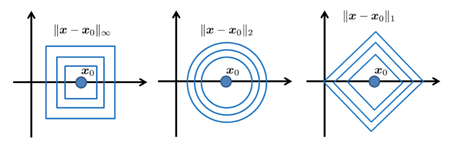
\includegraphics[scale=0.5]{Graphics/Norms.png}
\caption{Illustrations of norms.}
\label{fig:Norm}
\end{figure}
 
 
 
 
 
 
 
 S in FGSM is sign, which represents  \(L_{\infty}\) norm.
 Moosavi-Dezfooli et al.\cite{moosavi-dezfooli_deepfool_2016} proposed DeepFool to acquire the closest distance from the original input to the decision boundary of adversarial examples, which uses \(L_{2}\) norm to replace sign norm for a better result in image.
 \begin{center}
          \(x^{*} =x+\sigma\frac{\nabla_{x}J(x,y)}{\|\nabla_{x}J(x,y)\|_{2}} \)
\end{center}
 It could also be increased more broad norm, \(L_{\rho}\in [0,\infty)\):
 
 \(L_{1}\) norm as Manhattan metric to replace sign norm. 
 
 Liu et.al(\cite{liu_adversarial_2019}) proposed a new version of \(L_{2}\) norm named \(L_{2.5}\) norm, which is normalized \(L_{2}\) norm's result. 
\textit{Perturbation Selection and Adjustment} 
The attacker can use the network sensitivity information about the input differences to evaluate the dimensionality of the misclassification of the target that is most likely to cause the least interference. There are two types of perturbed input dimensions:

 \textbf{Perturb all the input dimensions}: Goodfellow et al.\cite{goodfellow_explaining_2015} proposed a method to perturb each input dimension, but there is a small amount of perturbation in the direction of the gradient sign calculated using the FGSM method. This method effectively minimizes the Euclidean distance between the original sample and the corresponding adversarial sample. 

\textbf{Perturb a selected input dimension}: Papernot et al.\cite{papernot_limitations_2015} choose to focus more on the complex process involving saliency mapping to perturbation by selecting only a limited number of input dimensions. The purpose of using a saliency map is to assign a value to a combination of input dimensions, which indicates whether the combination will contribute to adversarial goal if it is disturbed. This method effectively reduces the number of input features that are disturbed when making adversarial examples. In order to select the input dimensions that constitute the disturbance, all dimensions are sorted in descending order of adversarial saliency value. A legal example of the target class t is the saliency value  \(S(x,t)[i]\) of the component i of x, which is evaluated using the following equation:
\begin{equation}
S(x,t)[i]=\left\{
             \begin{array}{lr}
             0, & if \frac{\partial F_{t}}{\partial x_{i}}(x)\textless 0 \quad or \quad \sum_{j\neq t} \frac{\partial F_{t}}{\partial x_{i}}(x) \textgreater 0 \\
             \frac{\partial F_{t}}{\partial x_{i}}(x)\begin{vmatrix}
                \sum_{j\neq t} \frac{\partial F_{t}}{\partial x_{i}}(x)
                \end{vmatrix}, & otherwise\\
            
             \end{array}
\right.
\nonumber
\end{equation}
where \([\frac{\partial F_{t}}{\partial x_{i}}]_{ij}\) could be not difficultly derived from the Jacobian Matrix \(J_{F}\) of the victim model F. Input dimensions are added to perturbation \(\delta_{x}\) in the reducing order of the saliency values \(S(x,t)[i]\) until the acquiring image \(x_{*} = x + \delta x\) is misclassified by the network F.

The two perturbation selection types have their own assets and disadvantages. The first one is fine matched for the quick crafting of many adversarial examples rather with a larger perturbation, so it's more simple to tell the differences. The second one decreases the perturbations of relatively higher computation cost.

A better explanation of how LiDAR works, which is dealing with LiDAR signals in spherical coordinates \((r,\tau,\theta)\). In Figure \(\ref{fig:Lidar Rangeimage}\), Li et al.\cite{li_lidar_2020} used Velodyne UltraPuck to explain the principle of LiDAR. The vertical angle elevation for each laser beam is settled and the azimuth angle is determined by the scanning time and motor speed. Hence every range reading can be expressed by \(P_{i,j}=(\rho_{i,j},\tau_{i,j},\theta_{i,j}\), where i represents a certain laser beam and j is azimuth-angle index. Range readings fill into a predefined data buffer to complete range image. According to the azimuth and elevation of each point, it's easier to transform range image to point clouds.
  \begin{figure}[!htbp]
\centering
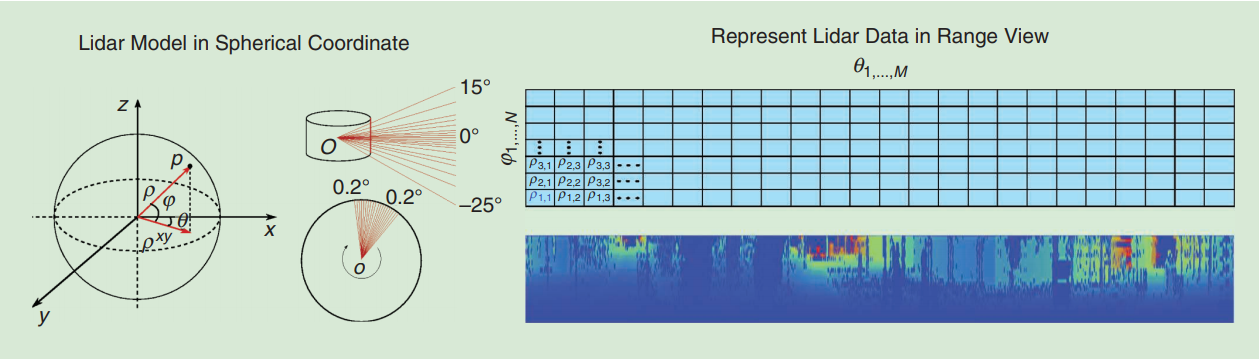
\includegraphics[scale=0.45]{Graphics/LIDAR RangeImage.png}
\caption{The range view of spinning lidar (Velodyne UltraPuck) for further processing. The range image (32 × 1,800) in pseudocolor facilitates the subsequent processing\cite{li_lidar_2020}}
\label{fig:Lidar Rangeimage}
\end{figure}
 
 One LiDAR point's azimuth and elevation is fixed. After perturbation to this point, LiDAR's physical characteristic should not be changed. As Figure \(\ref{fig:Adjustment}\) have shown one point named with "Original Point" is perturbated. When the perturbed point is green point, it have the same two angles as the original point. If perturbed point goes to red point, then the perturbed point's two angles should be adjusted to the original degrees, in order for keeping the physical character of LiDAR point clouds.
 \begin{figure}[!htbp]
\centering
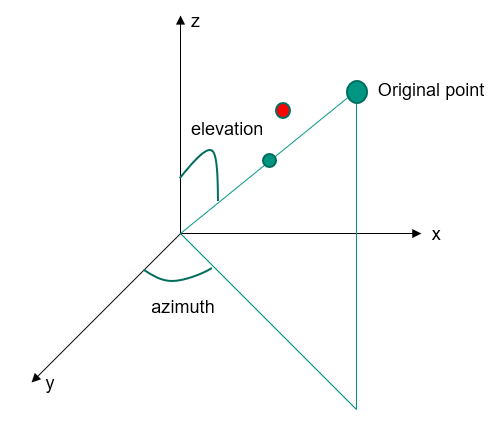
\includegraphics[scale=0.5]{Graphics/Adjustment.png}
\caption{LiDAR Point Coordinate System}
\label{fig:Adjustment}
\end{figure}

\paragraph{Defense Mechanism}
In this paper, defense strategy chosen to against the adversarial attacks is adversarial training, which is intuitive and widely accepted method.() The main idea is to inject \acrshort{fgsm}-generated advasarial samples into the training set in a manner that allows the trained model classify the adversarial examples correctly\cite{goodfellow_explaining_2015}. Formally, the loss function can be formulated as below:

\begin{equation}
          \widetilde{J}(\theta,x,y) = c J(\theta,x,y)+(1-c)J(\theta,x+\epsilon sign(\nabla_{x}J(\theta,x,y)),y)
\end{equation}
Where \(x\) represents the benign sample, \(c\) is a hyper parameter set to balance the accuracy of benign and adversarial samples, 


The prime propose of the adversarial training is to make the victim network more robust by adding adversarial samples to the training dataset. Adversarial training is a common brute force algorithm where the defense model easily produces lots of adversarial examples. The adversarial training is an argumentation process by injecting the adversarial examples. The training formular is given by \cite{goodfellow_explaining_2015}  

where J is initial loss function. The core intention behind this approach is to increase the robustness of the victim network by securing that it will classify the same category for precise as the perturbed examples. 

\subsubsection{Applications}
DNN is firstly developed in images. And FGSM as an efficient adversarial attack way is proposed firstly in neuron network in image classification. With the development of DNN, people is not satisfied only with image classification, there's more works and more networks are proposed to solve image segmentation and image detection for precise represent and complex scene. FGSM is then transferred to newer networks.
\paragraph{Image Semantic Segmentation}
Arnab et al.\cite{arnab_robustness_nodate} also evaluated FGSM and Iterative FGSM based adversarial attacks for semantic segmentation networks. Their work shows FGSM and its variants is also efficient in many semantic segmentation networks and pointed out that many attacks for classification do not straight transfer to segmentation mission. Cause the gradient can easily get from segmentation networks and FGSM just need the gradient to complete the attack. 
\paragraph{Image Object Detection}
Zhang et al.\cite{zhang_towards_2019} performs PGD(FGSM variant) as adversarial training method to defense object detectors, which can significantly improve the robustness and can defense adversarial examples generated by DAG\cite{xie_adversarial_2017} and RAP\cite{li_robust_2019}.

Liu et al.\cite{liu_mi-fgsm_2020} integrate MI-FGSM into target detection initially and achieve adequate attack performance, which attack method obtain higher success rate and more efficient and powerful than the attack algorithm such as PGD (Projected Gradient Descent) on object detection. They also show adversarial examples on Faster R-CNN\cite{ren_faster_2016} not only lead to misclassification, but there is also a wrong positioning, which is the wrong candidate boundary box. Those adversarial examples have established remarkable effects on black-box attack and white-box attack.

\paragraph{Point Cloud Segmentation}
PointNet and PointNet++ shows their elegant architecture and impressive results in point cloud classification mission. Liu et al.\cite{liu_extending_2019} transfer firstly FGSM attack and defenses to PointNet and PointNet++. They transfered with untargeted FGSM, targeted FGSM, FGSM's variants IFGSM, MIFGSM and PGD with 4 different gradient norms including \(L_{2.5}\) proposed by themselves. And also show the adversarial training is useful for defencing the adversarial attacks from FGSM and its variants.
\paragraph{FGSM in Point Cloud Object Detection}
With rapid development of LiDAR-based object detectors, the adversarial attacks on these networks is tiny. We plan to transfer FGSM and FGSM variants with 4 different fast gradient norms to attack and defense the detection model.
For perturbation selection part, different from images' 3 dimensions, LiDAR point clouds have 4 dimensions which are 4 features: \(x\) coordinate, \(y\) coordinate, \(z\) coordinate and intensity \(r\). So there are two different kinds of attack types: one is only attack one feature, which is separately attack \(x\) coordinate, \(y\) coordinate, \(z\) coordinate and intensity \(r\). The other is attack multiple features: \(xyz\) coordinates, and the combination of \(xyz\) coordinates and intensity \(r\). 


\subsection{Point Dropping}

\subsubsection{Critical Point Definition}

Different from multi-view networks and volumetric models, as the pioneer network as point-based method in point cloud classification shows their fast inference speed and capability of keeping more space information. PointNet\cite{qi_pointnet_2017} proved symmetric function could achieve permutation invariance to tackle the unordered problem of point clouds. They uses max-pooling layer as symmetric function to get points as global features. The gained points are called critical points.

Zheng et al.\cite{zheng_pointcloud_2019} proposed an adversarial method to drop the critical point compare with randomly point drop. The method of removing critical point shows its effectiveness with relative high sucess rate.
PointNet as a pioneer point-based network. Many subsequent networks pick it as the baseline. PointPillars\cite{lang_pointpillars_2019} is one of them. Although PointPillars uses the simplified PointNet, it can't get critical point by max-pooling layer and cause there is not max-pooling layer, but max layer in PointPillars.

\subsubsection{Critical Features in PointPillars}
 
PointNet shows the significant performance directly dealing with point clouds, which gives hug influences to subsequent point clouds based networks. PointPillars\cite{lang_pointpillars_2019} is one of them, which uses simplified PointNet\cite{qi_pointnet_2017} called Pillar Feature Net(Figure \(\ref{fig:Pillar Feature Net}\) have shown part of Pillar Feature Net) as one part of their work. Pillar Feature Net's first two step is import for definition of critical features. The first step is to stack points into pillars, the second step is to get learned features in each pillar. The learned features is defined by us as critical features.

\begin{figure}[!htbp]
\centering
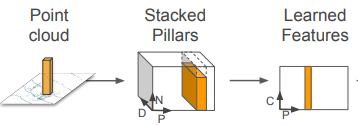
\includegraphics[scale=1]{Graphics/Pillar Feature Net.png}
\caption{Part of Pillar Feature Net\cite{lang_pointpillars_2019}}
\label{fig:Pillar Feature Net}
\end{figure}

\subsubsection{Definition of Critical Points in PointPillars}
If we want to drop critical point in PointPillars as Zheng\cite{zheng_pointcloud_2019} did in PointNet, we need to define critical points with critical features. As we know the process of PointPillars, it will get critical features per pillar. So the critical point we defined will also occur in each pillar. In OpenPCDet setting of PointPillars, there are 32 points per pillar and 64 features before max layer, after max layer through points dimension, there's 64 critical features per pillar left. We proposed two criterion for the definition of critical point based on this process:

1. Critical point in each pillar is the point with maximum critical feature value: After we get 64 critical features, we could obtain 1 maximal critical feature among these 64 critical features. The point, which contain the maximum critical feature value , corresponds to our criterion 1.

2. Critical point is the point that has most critical features. In operation of max layer, we've got 64 features. When we store the indexes of the maximal values, then we know how much critical features each point per pillar includes. We specify the point, which contains most number of critical features, as critical point based on our criterion 2.

In Figure \(\ref{fig:Critical Points}\), cells with critical features are pinpointed in colored background. In the whole table, 10 is the maximal critical feature value, and it's located at the third row, so this point is a critical point from first criterion. When counting the number of critical features, the fourth row has four colored cells, showing it has most features than other points. So, this point is a critical point based on second criterion.
\begin{figure}[!htbp]
\centering
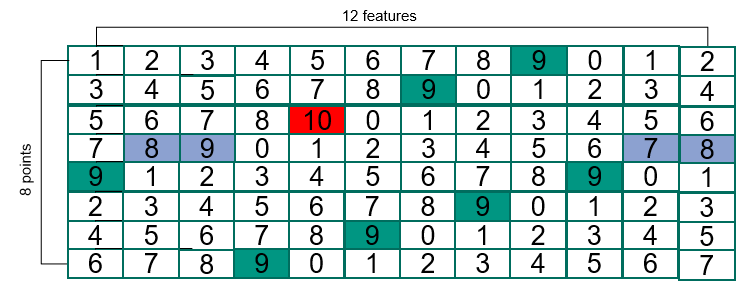
\includegraphics[scale=0.5]{Graphics/Critical Points.png}
\caption{Pseudo Process of Catching Critical Features}
\label{fig:Critical Points}
\end{figure}

\subsection{Common Perturbation Generation}
Hendrycks et al.\cite{hendrycks_benchmarking_2019} summarise the image processing methods and divided into image corruption and image perturbation. And build the ImageNet-C benchmark datasets and ImageNet-P benchmark datasets with these methods. There's 15 different corruption methods including Gaussian noise, shot noise, weather transfer, several blur methods, compression methods and etc. Each methods gives 5 levels to create 75 kinds of datasets. The perturbation methods contain motion blur, zoom blur, snow, brightness, translate, tilt(viewpoint variantion through 3D rotations), rotate and scale perturbations.

Inspired of Hendrycks, Michaelis et al.\cite{michaelis_benchmarking_2020} transfered this kind of work to autonomous driving datasets\cite{cordts_cityscapes_2016} rather than ImageNet\cite{deng_imagenet_2009}. As for creating methods, they selected only weather transfer methods for establishing "truly" datasets.
\subsubsection{Methods}
The weather transfer have been well developed in images. In images
 1. Add Gaussian noise perturbation.

2. Drop points randomly.

3. Add points surround cluster and ground points. Use RANSAC to segement ground points of lidar point clouds and then get clusters with DBSCAN. Random pick the some points in cluster and ground points to do the gaussian noise perturbation and then add the perturbated points to the original points as the addition of noise points.
\subsubsection{Simulation of adverse weather}
adverse weather is point clouds, which LiDAR acquired under adverse weather, including rain, snow, fog, etc. From Figure \(\ref{fig:Point Clouds Differences}\) we could seen in the point clouds under adverse weather are significant different with clean point clouds. 
\begin{figure}[!htbp]
    \centering
    \subfigure[Clean Point Cloud\cite{geiger_vision_2013}]{
        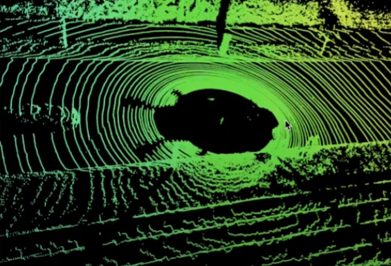
\includegraphics[width = \textwidth / 2 ]{Graphics/Clean Point Cloud.png}
        \label{fig:Clean Point Cloud}
    }
    \hspace{10pt}
     %add desired spacing between images, e. g. ~, \quad, \qquad, \hfill etc.
     %(or a blank line to force the subfigure onto a new line)
    \subfigure[Snow Point Cloud\cite{pitropov_canadian_2021}]{
        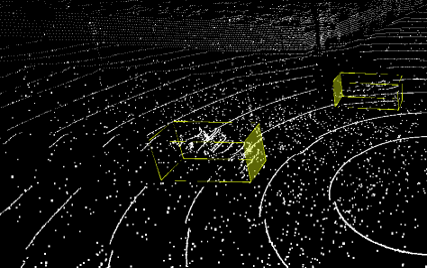
\includegraphics[width = \textwidth / 2 ]{Graphics/Snow Point Cloud.png}
        \label{fig:Snow Point Cloud}
    }
    \caption[Short Description for List of Figures]{The Differences between Clean Point Cloud and Snow Point Cloud}
    \label{fig:Point Clouds Differences}
\end{figure}

\textit{Creating methods in Point Clouds}: Considering establishing "truly" point clouds based on available point clouds. Gaussian noise could be occured in the process of LiDAR drawing point clouds\cite{gatt_micro-doppler_2000}. Merging with perturbation selection in FGSM we could get following method 1. LiDAR works like bat, which needs a emitter to emit laser beams, after some beams reflected by surface of objects, the receiver could received some of the reflected beam lasers. So the receiver could get nothing, which represents there's no points. Randomly drop points method means the dropped point cannot be received by the receiver. Weather transfer work is still not available in point cloud. And there's less creating methods than image domain.

1. Points perturbation with Gaussian noise applied with different features: intensity \(r\), \(xyz\) coordinates, and the combination of \(xyz\) coordinates and intensity \(r\).

2. Points randomly drop: in order to cause same influence to point cloud, the number of dropping points is getting from specific percentage of the total number of points.

\textit{Metric using benchmark datasets}
 To evaluate the robustness, rPP, which is the relative performance under point cloud perturbation, is used. rPP is the ratio of mPP and \(P_{clean}\):
\begin{center}
          \(rPP = \frac{mPP}{AP_{clean}} \)
\end{center}
\(P_{clean}\) is the average precision of the detection model under clean dataset, and mPP is the mean value of average precision of detection model under benchmark datasets:
\begin{center}
          \(mPC = \frac{1}{N_{C}}\sum_{c=1}^{N_{C}}\sum_{s=1}^{N_{S}}{AP_{C,S}} \)
\end{center}
\({P_{C,S}}\): performance evaluated on data changed with changes C with perturbation and drop points under severity level S

\({N_{C}}\): number of changes, including different methods

\({N_{S}}\): severity levels



\textit{Simulate Methods}

 
  \textit{Evaluation Metric: Weather Classification} 
 
 Vargas et.al\cite{vargas_rivero_weather_2020} have shown, use simple statistic parameters of point clouds: standard deviation and mean value of \(x\) coordinates and mean and standard deviation of echo-pulse width, which is intensity, etc. 13 parameters as input for a weather classifier.
 \textit{Evaluation Metric: Weather Points Semantic Segmentation Network}
 
 
 Evaluate the performance of simulation, weather point semantic segementation network is introduced. As the figure 6 shown, the DENSE\cite{DENSE} Dataset labeled each point cloud with a weather category, which is adverse weather consists of rain and fog. Heinzler et.al \cite{heinzler_cnn-based_2020} proposed WeatherNet training on DENSE Dataset. His results is shown in Table \(\ref{tab:DENSE}\)
 \begin{table}[h!]
  \begin{center}

    \begin{tabular}{|c|c|c|c|} % <-- Alignments: 1st column left, 2nd middle and 3rd right, with vertical lines in between
      \hline
      \multirow{2}{*}{Methods} & \multicolumn{3}{c|}{Weather Class}\\
    \cline{2-4}
       &\textbf{Clean(mIOU)} & \textbf{Rain(mIOU)}& \textbf{Fog(mIOU)}\\
      \hline
      WeatherNet & 93.35 & 90.92&88.81\\
      Cylinder3D & 98.91 & 94.61&91.63\\
      \color{blue}
      Delta & \color{blue}+5.56 & \color{blue}+3.69&\color{blue}+2.28\\
    \hline
    \end{tabular}
    \caption{Training Results on DENSE Dataset}
  \end{center}
    \label{tab:DENSE}
\end{table}
Cylinder3D\cite{zhu_cylindrical_2020} performs well in Semantic KITTI\cite{behley_semantickitti_2019}, which is an object semantic datasets. 

